\documentclass{beamer}
\usefonttheme[onlymath]{serif}
\usetheme{metropolis}

\usepackage[utf8]{inputenc}
\usepackage[sfdefault]{roboto}
\usepackage{graphicx}
\usepackage{amsmath}
\usepackage{amssymb}
\usepackage{multimedia}
\usepackage{graphicx}
\usepackage{minted}
\usepackage{transparent}
\usepackage{grid-system}

\newcommand{\norm}[1]{\left\| #1 \right\|}

\title{A Comparison of Denoising Methods for use in Super Resolution}
\author{Leanna Calla,\\Michael Stergianis}
\institute{University of Ontario Institute of Technology}
\date{\today}

\begin{document}
\frame{\titlepage}
\section{Introduction}
\begin{frame}
  \frametitle{Introduction}
  Super resolution is technique that combines low resolution images
  into high resolution images. Applications include
  \begin{itemize}
  \item medical imaging
  \item surveillance pictures and videos
  \item satellite images
  \end{itemize}
  A critical step in super resolution is
  often denoising an image.
\end{frame}
%
\section{Creating a dataset}
%
\begin{frame}
  \frametitle{Dataset}
  Noisy images were created with the following noising techniques
  \begin{itemize}
  \item salt \& pepper noise
  \item gaussian noise
  \item speckle noise
  \item poisson noise
  \end{itemize}
\end{frame}
%
\begin{frame}
  \frametitle{Dataset Example}
  The noise types were applied to the Matlab images, peppers and
  cameraman.
  \begin{figure}
    \centering
    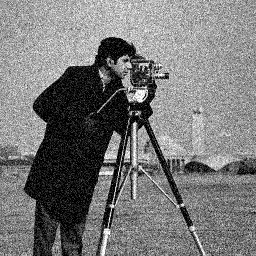
\includegraphics[width =
    0.35\textwidth]{../images/camera_noisy2.png}
    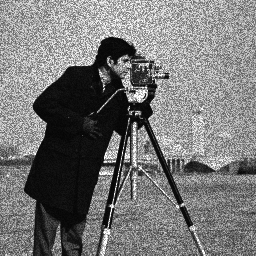
\includegraphics[width =
    0.35\textwidth]{../images/camera_noisy3.png}
    \caption{Left: Gaussian Noise. Right: Speckle Noise}
  \end{figure}
\end{frame}
%
\begin{frame}
  \frametitle{Dataset Example}

  \begin{figure}
    \centering
    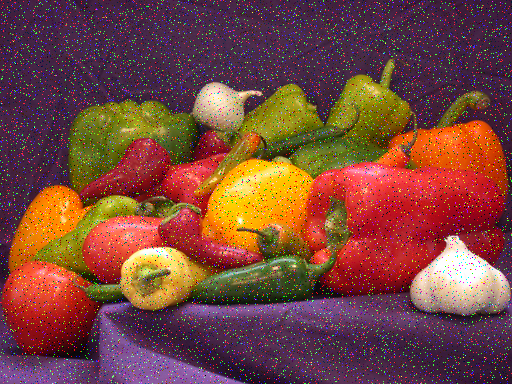
\includegraphics[width =
    0.35\textwidth]{../images/peps_noisy1.png}
    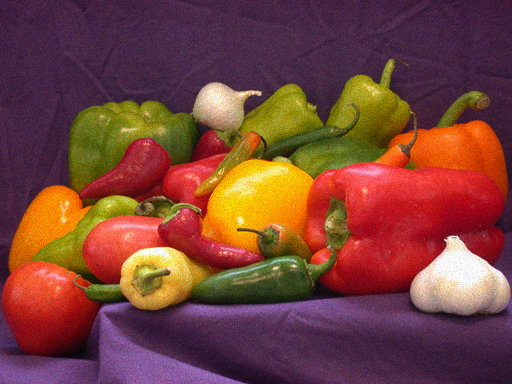
\includegraphics[width =
    0.35\textwidth]{../images/peps_noisy4.png}
    \caption{Left: Salt \& Pepper Noise. Right: Poisson Noise}
  \end{figure}
  
  
\end{frame}
%
\section{Filters}
%
\begin{frame}
  \frametitle{Gaussian Filtering}
  Gaussian filtering is a spatial blurring of the image.
  \[G_{\sigma}(\bar{x}) = \frac{1}{\sqrt{2 \pi \sigma^2}} \text{exp} \left(-
      \frac{\bar{x}^2}{2 \sigma^2}\right). \]
\end{frame}
%
\begin{frame}
  \frametitle{Testing Gaussian}
  \begin{figure}
    \centering
  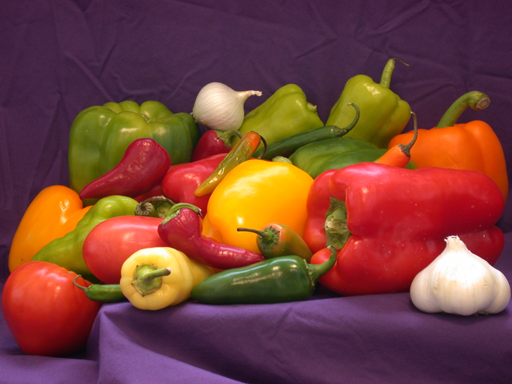
\includegraphics[width =
    0.25\textwidth]{../images/peps_truth.png}
    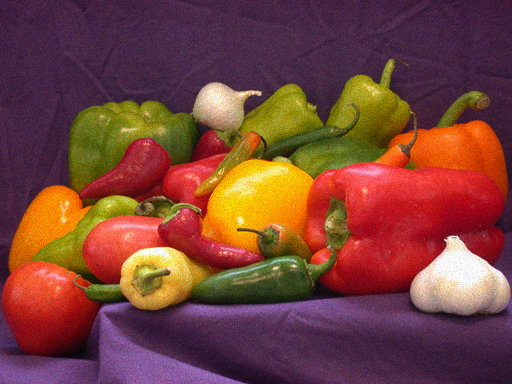
\includegraphics[width =
    0.25\textwidth]{../images/peps_noisy4.png}
    \includegraphics[width =
    0.25\textwidth]{../images/denoised/peps_noisy4_gaussian.png}
    \caption{Left to right: ground truth, Poisson noise, Gaussian
      filter on Poisson noise }
  \end{figure}
\end{frame}

\begin{frame}
  \frametitle{Bilateral Filtering}
  Bilateral filtering uses Gaussian blur, and takes into account
  effects of space and intensity parameters.
  \[ BF[I]_{\textbf{p}}= \displaystyle \frac{1}{W_p} \sum_{\textbf{q} \in S} G_{\sigma_s} \left(\norm{\textbf{p} - \textbf{q}}\right)
  G_{\sigma_r} \left(|I_{\textbf{p}} -
    I_{\textbf{q}}|\right)I_{\textbf{q}} \]

 \[ W_p = \sum_{\textbf{q} \in S} G_{\sigma_s} \left(\norm{\textbf{p} - \textbf{q}}\right)
   G_{\sigma_r} \left(|I_{\textbf{p}} - I_{\textbf{q}}|\right)\]
 
\end{frame}
%
\begin{frame}
  \frametitle{Testing Bilateral}
  \begin{figure}
    \centering
  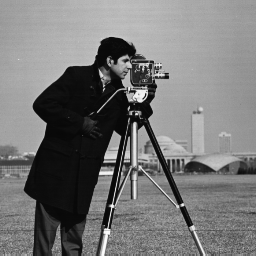
\includegraphics[width =
    0.25\textwidth]{../images/camera_truth.png}
    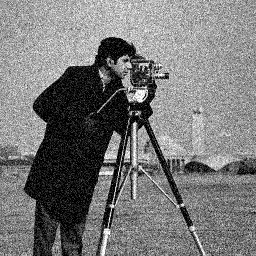
\includegraphics[width =
    0.25\textwidth]{../images/camera_noisy2.png}
    \includegraphics[width =
    0.25\textwidth]{../images/denoised/bilateral_backup/camera_noisy2_bilateral.png}
    \caption{Left to right: ground truth, Gaussian noise, bilateral
      filter on Gaussian noise }
  \end{figure}
  
\end{frame}

\begin{frame}
  \frametitle{Median Filtering}
  Two types of median filtering were explored
  \begin{itemize}
  \item Traditional median filter: the centre
    pixel of a sliding kernel is replaced with the median of the set
  \item Improved median filter: the centre pixel is replaced with the
    median as done in the traditional method, however the average of the
    kernel is then compared with the values within the kernel. This
    gives insight onto whether or not the kernel does indeed contain
    noise
  \end{itemize}
\end{frame}

\begin{frame}
  \frametitle{Testing Median Filters}
\begin{figure}
    \centering
  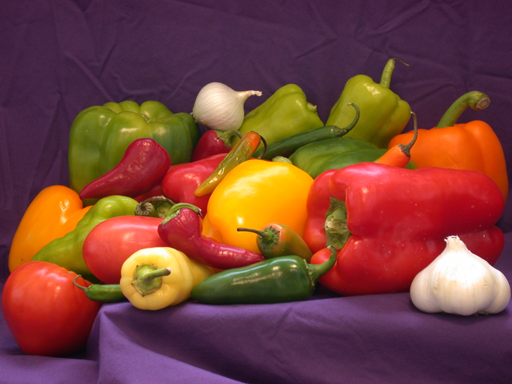
\includegraphics[width =
    0.22\textwidth]{../images/peps_truth.png}
    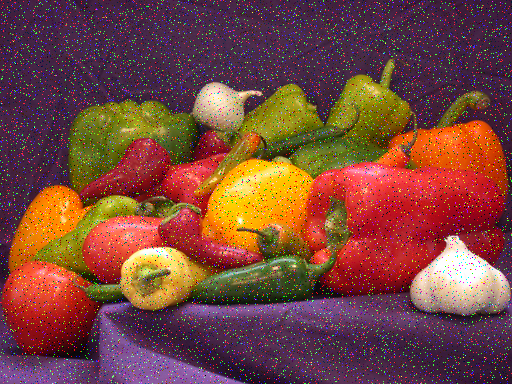
\includegraphics[width =
    0.22\textwidth]{../images/peps_noisy1.png}
    \includegraphics[width =
    0.22\textwidth]{../images/denoised/peps_noisy1_median.png}
    \includegraphics[width = 0.22\textwidth]{../images/denoised/peps_noisy1_improved_median}
    \caption{Left to right: ground truth, salt \& pepper noise, median
      filter on salt \& pepper noise, improved median on salt \&
      pepper noise }
  \end{figure}
\end{frame}

\begin{frame}
  \frametitle{Testing Median Filters}
\begin{figure}
    \centering
  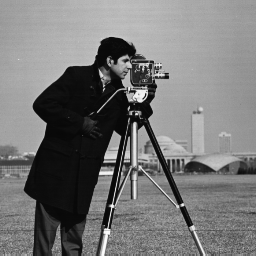
\includegraphics[width =
    0.22\textwidth]{../images/camera_truth.png}
    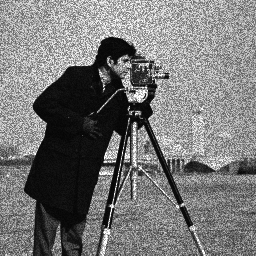
\includegraphics[width =
    0.22\textwidth]{../images/camera_noisy3.png}
    \includegraphics[width =
    0.22\textwidth]{../images/denoised/camera_noisy3_median.png}
    \includegraphics[width = 0.22\textwidth]{../images/denoised/camera_noisy3_improved_median}
    \caption{Left to right: ground truth, speckle noise, median
      filter on speckle noise, improved median on speckle noise }
  \end{figure}
\end{frame}

\section{Interpolation Techniques}
%
\begin{frame}
  \frametitle{Bilinear Interpolation}
  Bilinear interpolation is technique that traverses a 2D array by considering
  each direction separately, and combining them together with the following
  \[f(x, y) = \frac{1}{(x_2 - x_1)(y_2-y_1)} [x_2-x \quad x - x_1]
\begin{bmatrix} f(Q_{11}) & f(Q_{12}) \\ f(Q_{21}) & f(Q_{22}) \end{bmatrix} \begin{bmatrix} y_2 - y \\ y-y_1 \end{bmatrix}\]
\end{frame}

\section{Analysis}
%
\begin{frame}
  \frametitle{Tracking Statistics}
  Both the signal to noise ratio (SNR) and root mean square errors
  (RMSE) were computed. These values seem to depend on the filtering
  technique, as well as the noise type. Highlights are as follows
  \begin{itemize}
  \item Bilateral denoising had the lowest RMSE values overall
    \item Bilateral also has largest SNR values
    \item some negative values are seen for the SNR using improved
      median
    \end{itemize}
\end{frame}
%
\section{Conclusion}
%
\begin{frame}
  \frametitle{Conclusion}
Denoising is one of the many tasks required to use a super resolution
algorithm. We saw that while nonlinear filters often have longer
run times, they seem to perform best. 
\end{frame}

  
\end{document}
